%!TEX root = ../main.tex

\section{Численное исследование}

Была написана программа, реализующая разностную схему \eqref{sch:transition}, \eqref{sch:borders}. С помощью моделирования проверим полученные ранее теоретические результаты, а именно: устойчивость и сходимость схемы при выполнении условия устойчивости \eqref{cond:spectral_better}, а также свойства положений равновесия системы, описанные в разделе \ref{sec:theoretical_analysis}. Помимо этого, проверим поведение полной свободной энергии системы при моделировании.


\subsection{Вычислительный эксперимент: устойчивость}

Зафиксируем параметры уравнения \eqref{eq:one_dim}:
\begin{equation}
	\epsilon_0 = 0.2, \; \delta = 0.04, \; l = 1.0, \; \Gamma = 1.0, \; m = 0.5, \; K_\Phi = 4.8 \tpoint
	\label{exp:parameters}
\end{equation}
Перед нами случай <<сильного напряжения>> (см. выражение~\eqref{char:equilibriums}).

Моделируем решение в области 
\begin{equation}
	\clOmega = [0, W]_x \times [0, T]_t, \; W = 5, \; T = 1 \tpoint
	\label{exp:set}
\end{equation}

Зададим следующие краевые условия:
\begin{equation}
\begin{gathered}
	\phi(0, t) = 1, \; \phi(W, t) = 1 \tcomma \\
	\phi(x, 0) = \phi_0(x) = \begin{cases}
		1, \; \text{если} \; x \leqslant 2.25 \; \text{или} \; x \geqslant 2.75 \tsemicolon \\
		1 - 0.025 \cdot [1 + \cos(4 \pi x)], \; \text{если} \; 2.25 < x < 2.75 \tpoint
	\end{cases}
\end{gathered} \label{exp:borders}
\end{equation}
Обратим внимание, что $\phi_0(x)$ дважды дифференцируема всюду, кроме конечного числа точек, с ограниченной второй производной.

Обозначим $N_x$ число отрезков разбиения $[0, W]_x$ (узлов, соответственно, $N_x + 1$); $N_t$~-- число отрезков разбиения $[0, T]_t$. $h = W / N_x, \; \tau = T / N_t$.

\begin{figure}[!t]
	\centering
	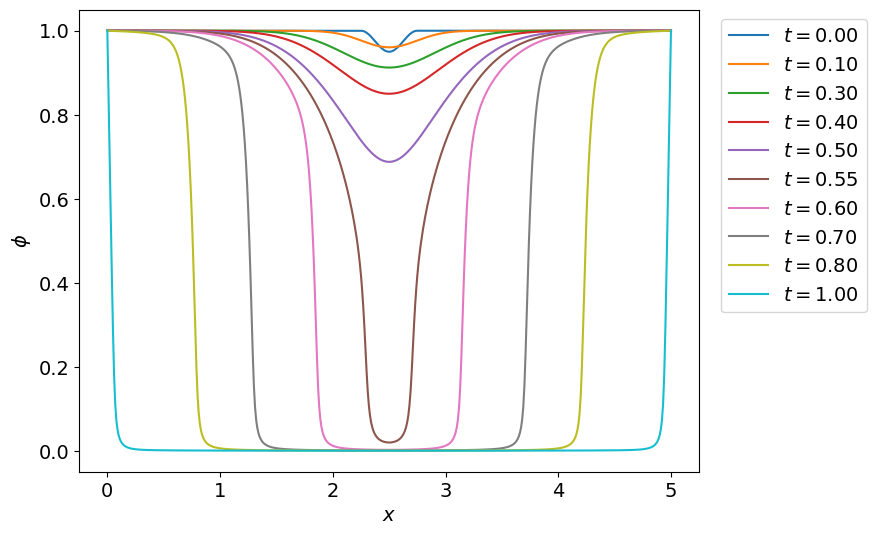
\includegraphics[width=\textwidth]{figures/typical_solution.png}
	\vspace{-0.8cm}
	\caption{Типичное решение задачи, $N_x = 10^3, \; N_t = 10^5$}
	\label{fig:typical_solution}
\end{figure}

Для начала посмотрим на типичное решение исследуемой задачи (рис.~\ref{fig:typical_solution}). Видно постепенное развитие канала электрического пробоя (разрушение среды) из небольшого начального возмущения фазового поля $\phi$ неповрежденной среды. Примерно в момент времени $t = 0.55$ канал пробоя <<прорастает насквозь>>, а именно: $\phi$ вблизи точки $x = 2.5$ приближается к нулевому значению. Обратим внимание, что в период времени $t \in (0.3, \; 0.55)$ канал пробоя (область, где $\phi$ существенно отличается от $1$) практически не растет в ширину, а при $t > 0.55$, напротив, растет в ширину почти с постоянной скоростью.

Проверим полученную в предыдущем разделе оценку \eqref{cond:spectral_better} устойчивости разностной схемы. Будем считать, что в вычислительном эксперименте схема неустойчива, если программа завершилась с ошибкой: произошло деление на~$0$ (в формуле \eqref{eq:epsilon} функции $\epsilon(\phi)$ при $f(\phi) = -\delta$) или значения $\phi$ ушли на бесконечность (переполнился тип double). Будем перебирать $N_x$ и $N_t$, запоминая пары соседних точек, в одной из которых устойчивость есть, а в другой нет. Так получим опытную оценку устойчивости схемы. Отобразим ее на графике вместе с оценкой \eqref{cond:spectral_better} (рис. \ref{fig:stability_bounds}).

Эксперимент показывает, что оценка \eqref{cond:spectral_better} удачна: она примерно повторяет контур опытной оценки, к тому же ее график лежит выше, то есть она имеет некоторый <<запас>> до момента, когда в программе возникает ошибка. Именно ради этого <<запаса>> знаменатель исходной оценки  \eqref{cond:spectral_better_theoretical} был удвоен.

\begin{figure}[!t]
	\centering
	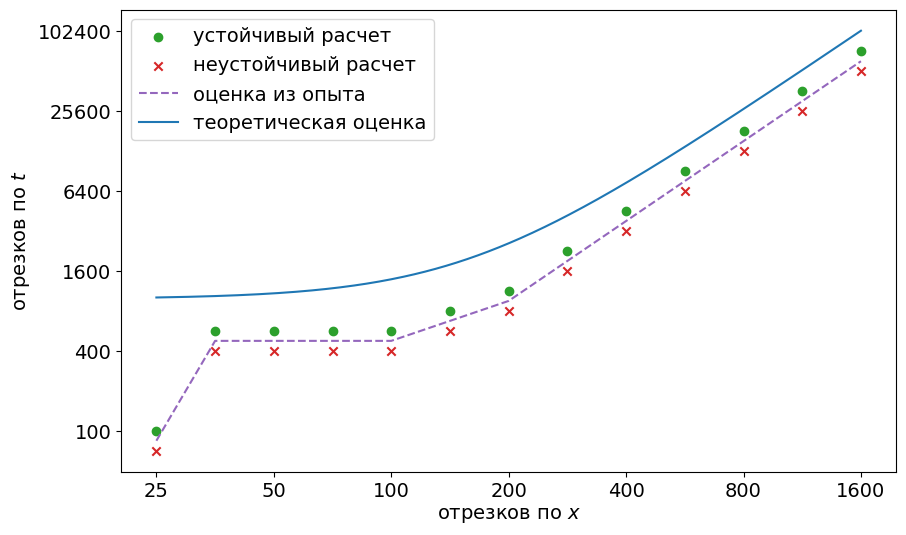
\includegraphics[width=\textwidth]{figures/stability_bounds.png}
	\vspace{-0.7cm}
	\caption{Теоретическая и опытная оценки устойчивости разностной схемы}
	\label{fig:stability_bounds}
\end{figure}


\subsection{Вычислительный эксперимент: сходимость}

Аппроксимация разностной схемой \eqref{sch:transition}, \eqref{sch:borders} дифференциальной задачи~\eqref{eq:one_dim},~\eqref{eq:one_dim_initial},~\eqref{eq:one_dim_marginal} очевидна; для устойчивости схемы в ходе нестрогого анализа получено условие \eqref{cond:spectral_better}, применимое на практике. Теперь экспериментально проверим сходимость.

На множестве $C_2(\clOmega)$ дважды непрерывно дифференцируемых функций в замкнутой области $\clOmega = [0, W]_x \times [0, T]_t$ рассмотрим следующие нормы: равномерную $\enorm_C$ и $L_2$-норму $\enorm_2$.
$$\norm{f}_C = \max \limits_{(x, t) \in \clOmega} |f(x, t)|; \qquad \norm{f}_2 = \sqrt{\int \limits_{\clOmega} f^2(x, t) dx dt} \tpoint$$

Теперь рассмотрим регулярную сетку $\Omega_{h, \tau} \subset \clOmega$ с некоторой зависимостью $\tau = \tau(h)$. Ограничивая функции из $C_2(\Omega)$ на сетке $\Omega_h = \Omega_{h, \tau(h)}$, получаем множество $C_2(\clOmega)_h$ сеточных функций.

На множестве $C_2(\clOmega)_h$ сеточных функций введем нормы, согласованные с $\enorm_C$ и $\enorm_2$:
$$\norm{f_j^k}_C = \max \limits_{(j, k) \in \Omega_h} |f_j^k|; \qquad \norm{f_j^k}_2 = \sqrt{h \tau \sum \limits_{(j, k) \in \Omega_h} (f_j^k)^2} \tpoint$$

Перейдем к вычислительному эксперименту. Сходимость будем проверять по описанным выше нормам $\enorm_C$ и $\enorm_2$ на множестве сеточных функций. Так как аналитическое решение дифференциальной задачи неизвестно, будем сравнивать ряд результатов на все более мелких сетках по норме с лучшим результатом в ряду. При сравнении функцию на более мелкой сетке ограничиваем на более крупной, игнорируя часть узлов.

Зафиксируем ранее использовавшиеся параметры уравнения \eqref{exp:parameters}, \eqref{exp:set}; зададим краевые условия \eqref{exp:borders}. Положим $N_x = W / h$~-- число отрезков разбиения по $x$, $N_t = T / \tau$~-- по $t$.

Во всех описанных далее вариантах расчетов соблюдается условие устойчивости~\eqref{cond:spectral_better}.

Для начала зафиксируем $N_x = 200$ и будем перебирать $N_t$, каждый раз увеличивая его вдвое. Сравнение по нормам с результатом при $N_t = 204800$ изображено на рис. \ref{fig:convergence_fixed_nx}. Разностная схема имеет первый порядок аппроксимации по $t$; опыт показывает первый порядок сходимости $\bigO (\tau)$.

Зафиксируем $N_t = 204800$ и будем перебирать $N_x$, каждый раз увеличивая его вдвое. Сравнение по нормам с результатом при $N_x = 1600$ изображено на рис. \ref{fig:convergence_fixed_nt}. Разностная схема имеет второй порядок аппроксимации по $x$; опыт показывает второй порядок сходимости $\bigO (h^2)$.

\begin{figure}[!tp]
	\centering
	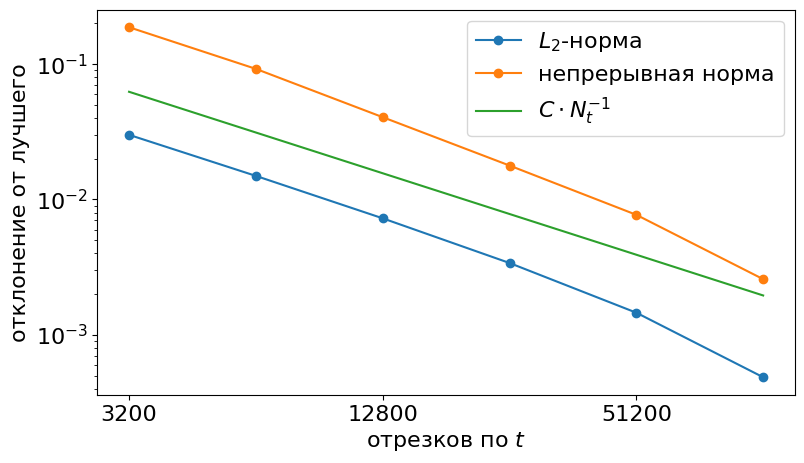
\includegraphics[width=0.72\textwidth]{figures/convergence_fixed_nx.png}
	\vspace{-0.2cm}
	\caption{Ошибка решения по норме при фиксированном $N_x = 200$}
	\label{fig:convergence_fixed_nx}
	\vspace{0.6cm}
	
	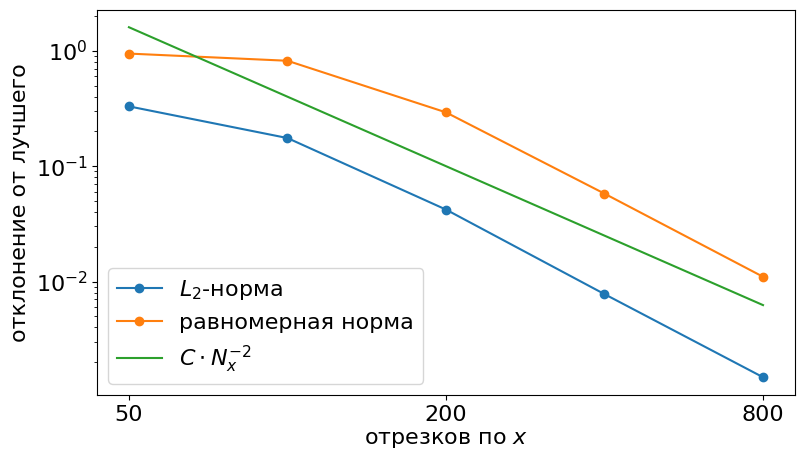
\includegraphics[width=0.72\textwidth]{figures/convergence_fixed_nt.png}
	\vspace{-0.2cm}
	\caption{Ошибка решения по норме при фиксированном $N_t = 204800$}
	\label{fig:convergence_fixed_nt}
	\vspace{0.6cm}
	
	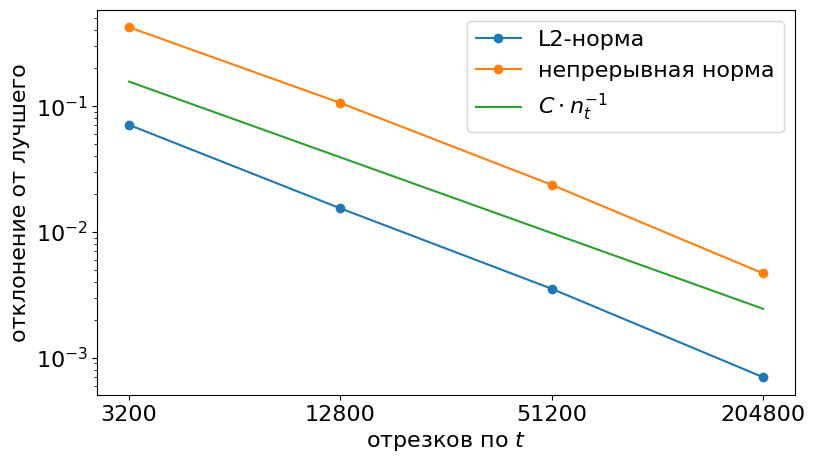
\includegraphics[width=0.72\textwidth]{figures/convergence_connected.png}
	\vspace{-0.2cm}
	\caption{Ошибка решения по норме при $N_t = 0.08 \cdot N_x^2$}
	\label{fig:convergence_connected}
\end{figure}

Теперь свяжем $N_x$ и $N_t$ уравнением, так чтобы при $h, \tau \to 0$ выполнялось условие устойчивости \eqref{cond:spectral_better}. При выбранных параметрах модели подойдет $N_t = 0.08 \cdot N_x^2$. Аналогично проведем сравнение ряда измерений по норме с лучшим (рис. \ref{fig:convergence_connected}). Как и ожидалось, измерения показывают сходимость $\bigO (\tau + h^2) = \bigO (\tau)$ первого порядка по времени при выбранном уравнении связи.

В первых двух опытах, без стремления обоих шагов сетки к $0$, последовательности сеточных функций имели неясный предел. В третьем же, если принять предположение об устойчивости разностной схемы, сеточные функции сходятся к решению дифференциальной задачи \eqref{eq:one_dim}, \eqref{eq:one_dim_initial}, \eqref{eq:one_dim_marginal}.


\subsection{Вычислительный эксперимент: \\ положения равновесия}

Ранее были исследованы положения равновесия уравнения \eqref{eq:one_dim} вида $\phi \hm \equiv C$. Их количество и устойчивость определяются значением выражения \eqref{char:equilibriums} (обозначено $\xi$). Проверим этот результат экспериментально.

Зададим модели параметры \eqref{exp:parameters}, \eqref{exp:set}, $K_\Phi$ определим позже. В качестве начального условия берем возмущенное положение равновесия: $\phi(x, 0) = C \hm + A \cos(\omega x); \; \phi(0, t) = \phi(0, 0), \; \phi(W, t) = \phi(W, 0)$. Амплитуда $A$ мала, порядка~$0.01$. $N_x = 800, \; N_t = 51200$.

Если положение равновесия устойчиво, то при любом $\omega$ возмущение угасает; если неустойчиво, то существует некоторое $\omega_0$, такое что при $\omega < \omega_0$ возмущение растет.

Положим $K_{\Phi, 1} = 0, \; K_{\Phi, 2} = 1.1, \; K_{\Phi, 3} = 4.8$. Было задано $\delta = 0.04$. В таком случае $\xi_1 = 0 < \delta^2, \; \xi_2 = 0.121 \in (\delta^2, (1 + \delta)^2), \; \xi_3 = 2.304 > (1 + \delta)^2$.

Вначале рассмотрим $K_{\Phi, 1} = 0, \; \xi_1 < \delta^2$~-- случай <<слабого напряжения>>. Система имеет два положения равновесия: $\phi \equiv 0$ неустойчивое, $\phi \equiv 1$ устойчивое. На рис. \ref{fig:equilibrium_1_0}, \ref{fig:equilibrium_1_1} видно теоретически предсказанное поведение возмущенной среды: при $C = 0$ возмущение растет, при $C = 1$~-- затухает. В точке $C = 0$ производная функции $\chi(\phi)$ (см. выражение \eqref{eq:equilibruim_characteristic}) равна $0$, поэтому, чтобы увидеть рост возмущения, приходится брать небольшое $\omega$, обеспечивая небольшое значение $\partflxx{\phi}$. В эксперименте с $\phi \equiv 1$ взято $C = 1 - A$, чтобы значения $\phi$ не превосходили $1$.

\begin{figure}[!t]
	\centering
	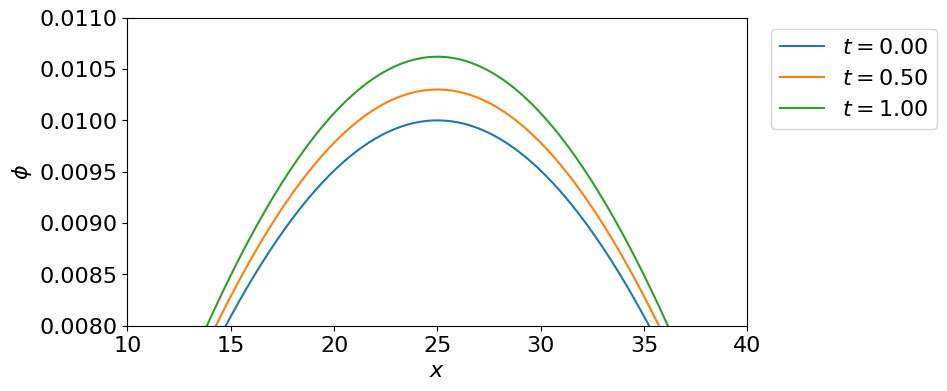
\includegraphics[width=0.9\textwidth]{figures/equilibrium_1_0.png}
	\vspace{-0.3cm}
	\caption{Случай <<слабого напряжения>>: возмущенное положение равновесия $\phi \equiv 0$, неустойчивое}
	\label{fig:equilibrium_1_0}
	\vspace{0.5cm}
	
	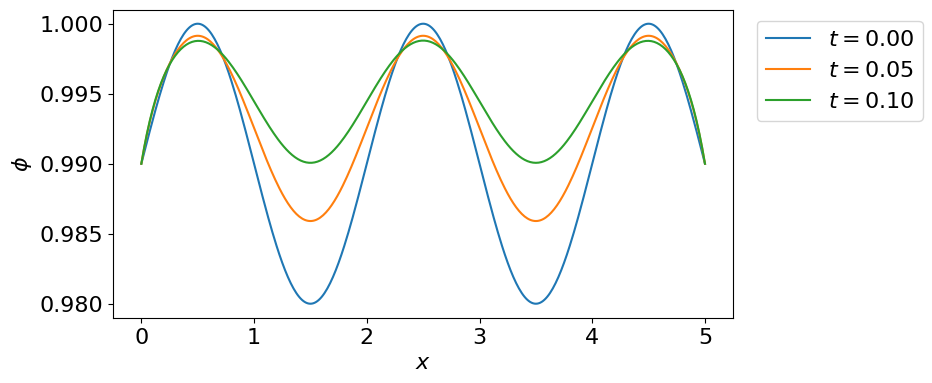
\includegraphics[width=0.9\textwidth]{figures/equilibrium_1_1.png}
	\vspace{-0.3cm}
	\caption{Случай <<слабого напряжения>>: возмущенное положение равновесия $\phi \equiv 1$, устойчивое}
	\label{fig:equilibrium_1_1}
\end{figure}

Теперь рассмотрим $K_{\Phi, 2} = 1.1, \; \xi_2 \in (\delta^2, (1 + \delta)^2)$~-- случай <<среднего напряжения>>. Система имеет три положения равновесия: $\phi \equiv 0$ устойчивое, $\phi \equiv C_3 \approx 0.5$ неустойчивое ($C_3$~-- корень функции $\chi(\phi)$ в интервале $(0, 1)$), $\phi \equiv 1$ устойчивое. Поведение возмущенной среды изображено на \linebreak рис. \ref{fig:equilibrium_2_0}, \ref{fig:equilibrium_2_05}, \ref{fig:equilibrium_2_1}, оно соответствует теоретическим результатам.

\begin{figure}[!tp]
	\centering
	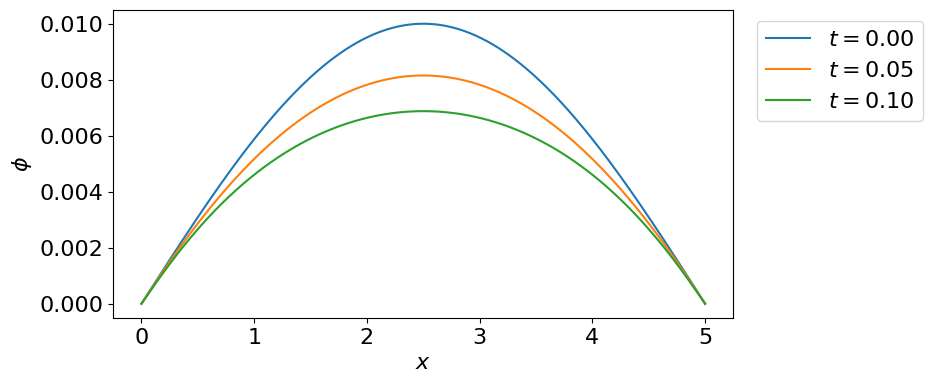
\includegraphics[width=0.9\textwidth]{figures/equilibrium_2_0.png}
	\vspace{-0.3cm}
	\caption{Случай <<среднего напряжения>>: возмущенное положение равновесия $\phi \equiv 0$, устойчивое}
	\label{fig:equilibrium_2_0}
	\vspace{0.5cm}

	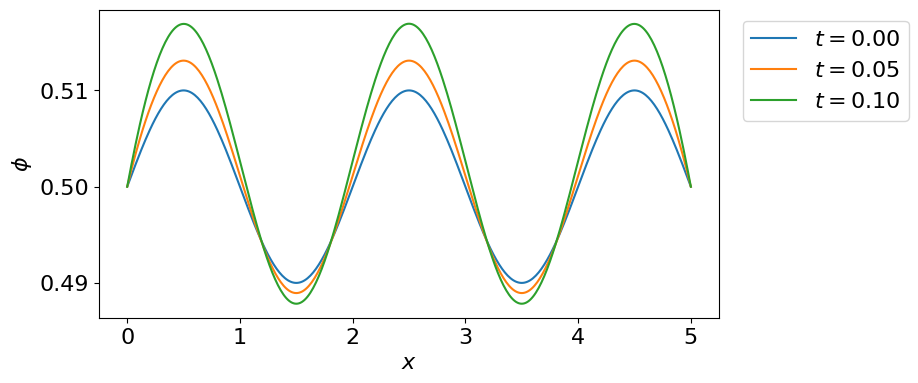
\includegraphics[width=0.9\textwidth]{figures/equilibrium_2_05.png}
	\vspace{-0.3cm}
	\caption{Случай <<среднего напряжения>>: возмущенное положение равновесия $\phi \equiv C_3 \approx 0.5$, неустойчивое}
	\label{fig:equilibrium_2_05}
	\vspace{0.5cm}
	
	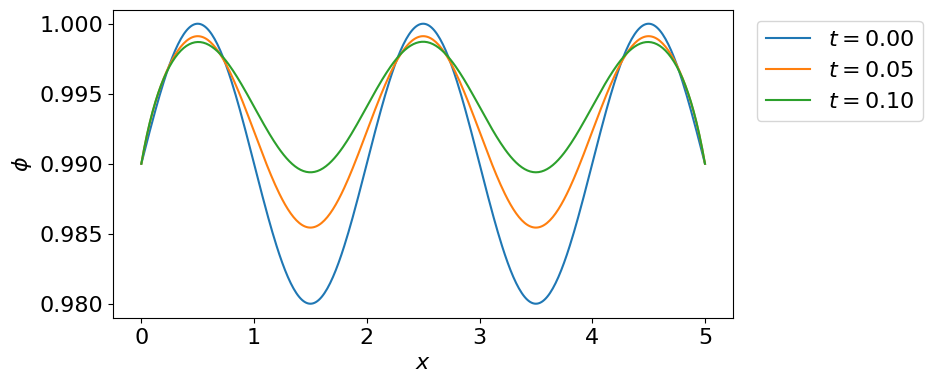
\includegraphics[width=0.9\textwidth]{figures/equilibrium_2_1.png}
	\vspace{-0.3cm}
	\caption{Случай <<среднего напряжения>>: возмущенное положение равновесия $\phi \equiv 1$, устойчивое}
	\label{fig:equilibrium_2_1}
\end{figure}

Наконец, рассмотрим $K_{\Phi, 3} = 4.8, \; \xi_3 > (1 + \delta)^2$~-- случай <<сильного напряжения>>. Система имеет два положения равновесия: $\phi \equiv 0$ устойчивое, $\phi \equiv 1$ неустойчивое. Поведение возмущенной среды изображено на рис. \ref{fig:equilibrium_3_0}, \ref{fig:equilibrium_3_1}, оно также соответствует теории.

\begin{figure}[!t]
	\centering
	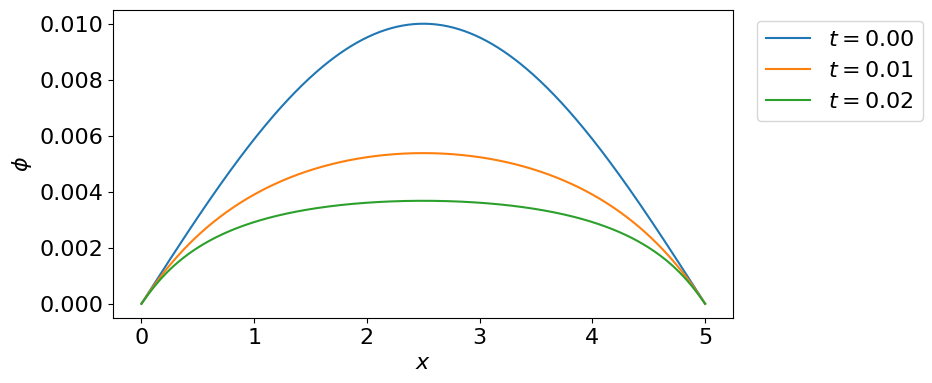
\includegraphics[width=0.9\textwidth]{figures/equilibrium_3_0.png}
	\vspace{-0.3cm}
	\caption{Случай <<сильного напряжения>>: возмущенное положение равновесия $\phi \equiv 0$, устойчивое}
	\label{fig:equilibrium_3_0}
	\vspace{0.5cm}
	
	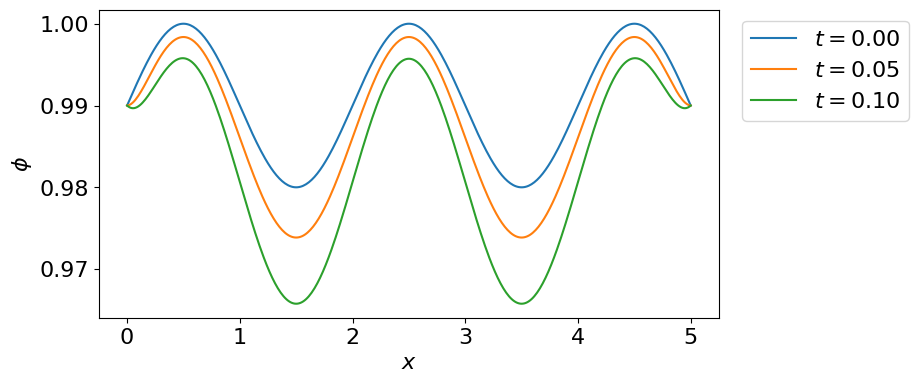
\includegraphics[width=0.9\textwidth]{figures/equilibrium_3_1.png}
	\vspace{-0.3cm}
	\caption{Случай <<сильного напряжения>>: возмущенное положение равновесия $\phi \equiv 1$, неустойчивое}
	\label{fig:equilibrium_3_1}
\end{figure}


\subsection{Вычислительный эксперимент: свободная энергия}

В рассматриваемой модели введена функция свободной энергии \eqref{eq:energy}, заданная интегралом плотности свободной энергии \eqref{eq:energy_density} по пространству.

Построим график полной свободной энергии системы от времени. Зададим модели параметры \eqref{exp:parameters}, \eqref{exp:set} и краевые условия \eqref{exp:borders}. Ранее мы уже проводили расчеты в этой конфигурации~-- графики $\phi$ изображены на рис. \ref{fig:typical_solution}.

Единственное существенное дополнение, требующееся использованной ранее схеме \eqref{sch:transition}, \eqref{sch:borders},~-- вычисление разностной производной $\partial_h \phi_i^j / \partial_h x$. Ограничимся простейшей разностной производной первого порядка, так как искомая величина не влияет на пересчет состояния системы.

Результат вычисления полной свободной энергии $\Pi$ в зависимости от времени изображен на рис. \ref{fig:energy}. Для сравнения с рис. \ref{fig:typical_solution} пунктирными линиями соответствующих цветов отмечены моменты времени. Интересно, что до момента $t = 0.5$ энергия $\Pi$ убывает очень медленно; после, при $t \approx 0.55$, резко падает; затем падение замедляется, и после $t = 0.6$ убывание выравнивается, становясь близким к линейному; так продолжается практически до полного разрушения среды.

\begin{figure}
	\centering
	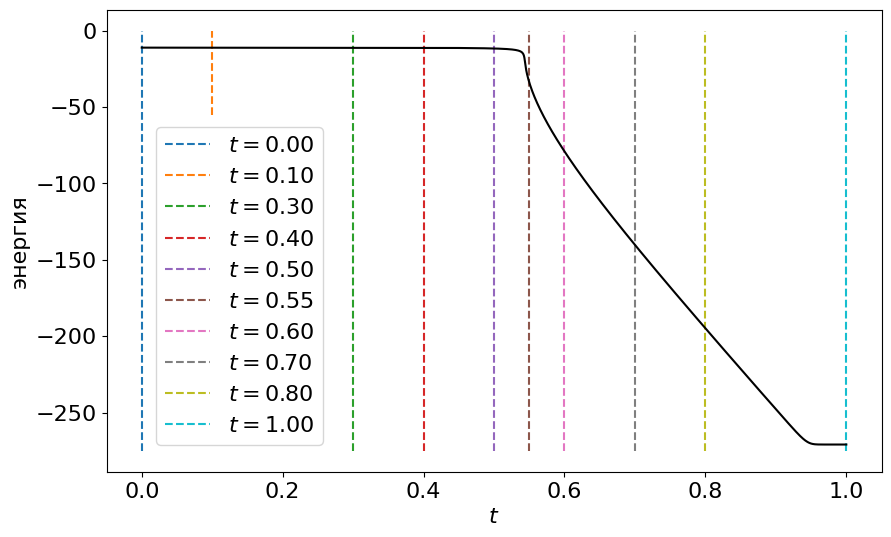
\includegraphics[width=\textwidth]{figures/energy_total.png}
	\vspace{-0.6cm}
	\caption{Поведение полной свободной энергии системы}
	\label{fig:energy}
\end{figure}

Отметим, что вывод системы уравнений \eqref{eq:Phi}, \eqref{eq:phi} динамики системы из выражений \eqref{eq:energy}, \eqref{eq:energy_density} для свободной энергии означает, что система в ходе эволюции стремится в положение с как можно меньшей свободной энергией. Поэтому для адекватного моделирования системы крайне важно, чтобы полная свободная энергия $\Pi$ не возрастала. Мы не дали этому теоретического обоснования для используемой разностной схемы, однако проверили на опыте. Другими словами, это означает, что при используемом виде краевых условий и параметрах расчета предложенная схема является градиентно-устойчивой.